\documentclass{llncs}
% \documentclass[twocolumn]{article}

% \usepackage{latexsym}
% \usepackage{amssymb}
\usepackage{graphicx}
% \usepackage{cite}
% \usepackage{url}
% \usepackage{soul}
% \usepackage{multirow}
% \usepackage{listings}
% \setstcolor{red}
% \usepackage[utf8]{inputenc}
% \usepackage[T1]{fontenc}

% \usepackage{comment}
% \usepackage{times}

%%%%%%%%%%%%%%%%%%%%%%%%%%%%%%%%%%%%%%%%%%%%%%%%%%%%%%%%%%%%%%%%%%%%%%%

\newcommand{\hcinv}{\texttt{hc\_inversion}\xspace}
\newcommand{\coqdockw}[1]{\texttt{#1}}
\newcommand{\inversion}{\coqdockw{inversion}\xspace}
\newcommand{\inv}{\coqdockw{inv}\xspace}
\newcommand{\simlight}{\texttt{Simlight}\xspace}
\newcommand{\compcert}{\texttt{CompCert}\xspace}
\newcommand{\clight}{\texttt{Clight}\xspace}
\newcommand{\simsoc}{\texttt{SimSoC}\xspace}
\newcommand{\simsoccert}{\texttt{SimSoC-Cert}\xspace}
\newcommand{\stt}{\small\tt}
\newcommand{\why}{\texttt{Why}\xspace}
\newcommand{\whyML}{\texttt{WhyML}\xspace}
\newcommand{\whyCert}{\texttt{WhyCert}\xspace}
\newcommand{\framac}{\texttt{Frama-C}\xspace}


%replace XXX with the submission number you are given from the ASPLOS submission site.
\usepackage[normalem]{ulem}
\usepackage{xspace}
\usepackage{alltt}
\usepackage{amsmath}
\usepackage{extarrows}


%\setlength{\intextsep}{10pt plus 2pt minus 2pt}

\begin{document}
%date not printed
\date{}

\title{SimSoC: A Fast, Proven Faithful, Full System Virtual Prototyping Framework}
\author{Vania Joloboff\inst{1} \and Jean\--Francois Monin\inst{2}
   \and Xiaomu Shi\inst{3}}
\institute{East China Normal University, Shanghai, China, INRIA, France\\
\email{vania.joloboff@inria.fr},\\
\and Grenoble University, France,\\
\email{jean-francois.monin@imag.fr},\\
\and Tsinghua University, China,\\
\email{xmshi@tsinghua.edu.cn}
}
\maketitle
\thispagestyle{empty}

\begin{abstract}

  This paper presents the SimSoC virtual prototyping framework, a full
  system simulation framework, based on SystemC and Transaction Level
  Modeling. SimSoC takes as input a binary executable file, which can
  be a full operating system, and simulates the behavior of the target
  hardware on the host system. It is using internally dynamic binary
  translation from target code to host code to simulate the
  application software. A potential issue with simulators is that they
  might not accurately simulate the real hardware. We aimed at
  filling this gap by proving that the ARM instruction set simulator
  coded in C is a high fidelity implementation of the ARM
  architecture, using the Coq theorem prover, and starting from a
  formal architectural model in Coq. The first part of the paper
  presents the general architecture of SimSoC.  The second part
  describes the proof of the ARM simulator.
\end{abstract}

\section{Introduction}

The SimSoC project is developing a simulation framework geared towards
full system simulation, able to simulate complete System-on-Chips or
boards. A platform simulator is typically mixing hardware components
models (e.g. a network controller) with one or more processor
Instruction Set Simulators (ISS). To this end, SimSoC combines
SystemC/TLM models for new IP’s and interconnects, with one or more
ISS. Each ISS is designed as a SystemC module that issues transactions
towards the other models.  In this paper, we present the overall
system architecture and the ISS technology. To achieve fast processor
simulation, the SimSoC ISS technology uses a form of dynamic
translation, using an intermediate representation and pre-generated
code using specialization, a technique already used within virtual
machines.  The hardware models are standard SystemC TLM abstractions
and the simulator uses the standard SystemC kernel. Therefore, the
simulation host can be any commercial off-the-shelf computer
and yet provide reasonable simulation performance.

A platform simulator such as SimSoC can be used to test critical
software such as cryptography or safety related embedded software.  In
these situations, it is necessary to work with the full system
implementation, not only with the model specification. It is also
important to use a very faithful simulator in order to ensure that no
bias is introduced.  To achieve that goal, we have worked to
demonstrate how it can be certified that the simulated execution of a
binary program on the Instruction Set Simulator of a target
architecture indeed produces the expected result. This actually
requires several steps, to prove first that the translation from C
code to machine code is correct, and second that the simulation of the
machine code is also correct, that is, they all preserve the semantics
of the source code; together with the fact that all of these proofs
are verified using a theorem prover or proof checker, not subject to
human error in the proof elaboration or verification. The end result
is a faithful simulator.

The first part of this paper describes the generic architecture of the
SimSoC framework with discussion of speed and accuracy.  The second
part of the paper describes how we have developed a faithful,
certified simulator. The technique presented here partly relies on
already existing tools, in particular the Coq proof assistant, the
\compcert C compiler, a certified compiler for the C language, combined
with our own work to prove the correctness of an ARM Instruction Set
Simulator, integrated within SimSoC.


\section{The SimSoC framework}

An instruction-set simulator (ISS) is used to mimic the behavior of a
target computer processor on a simulation host machine. The main task
of an ISS is to carry out the computations that correspond to each
instruction of the simulated program. There are several alternatives
to achieve such simulation. In {\em interpretive simulation}, each
instruction of the target program is fetched from memory, decoded, and
executed. This technique has been used in popular ISS's such as
Simplescalar~\cite{simplescalar-1997}. It is flexible and easy to
implement, but the simulation speed is slow as it wastes a lot of time
in decoding. A faster technique to implement an ISS is {\em dynamic
  binary translation}.
\begin{figure}[th]
  \centering
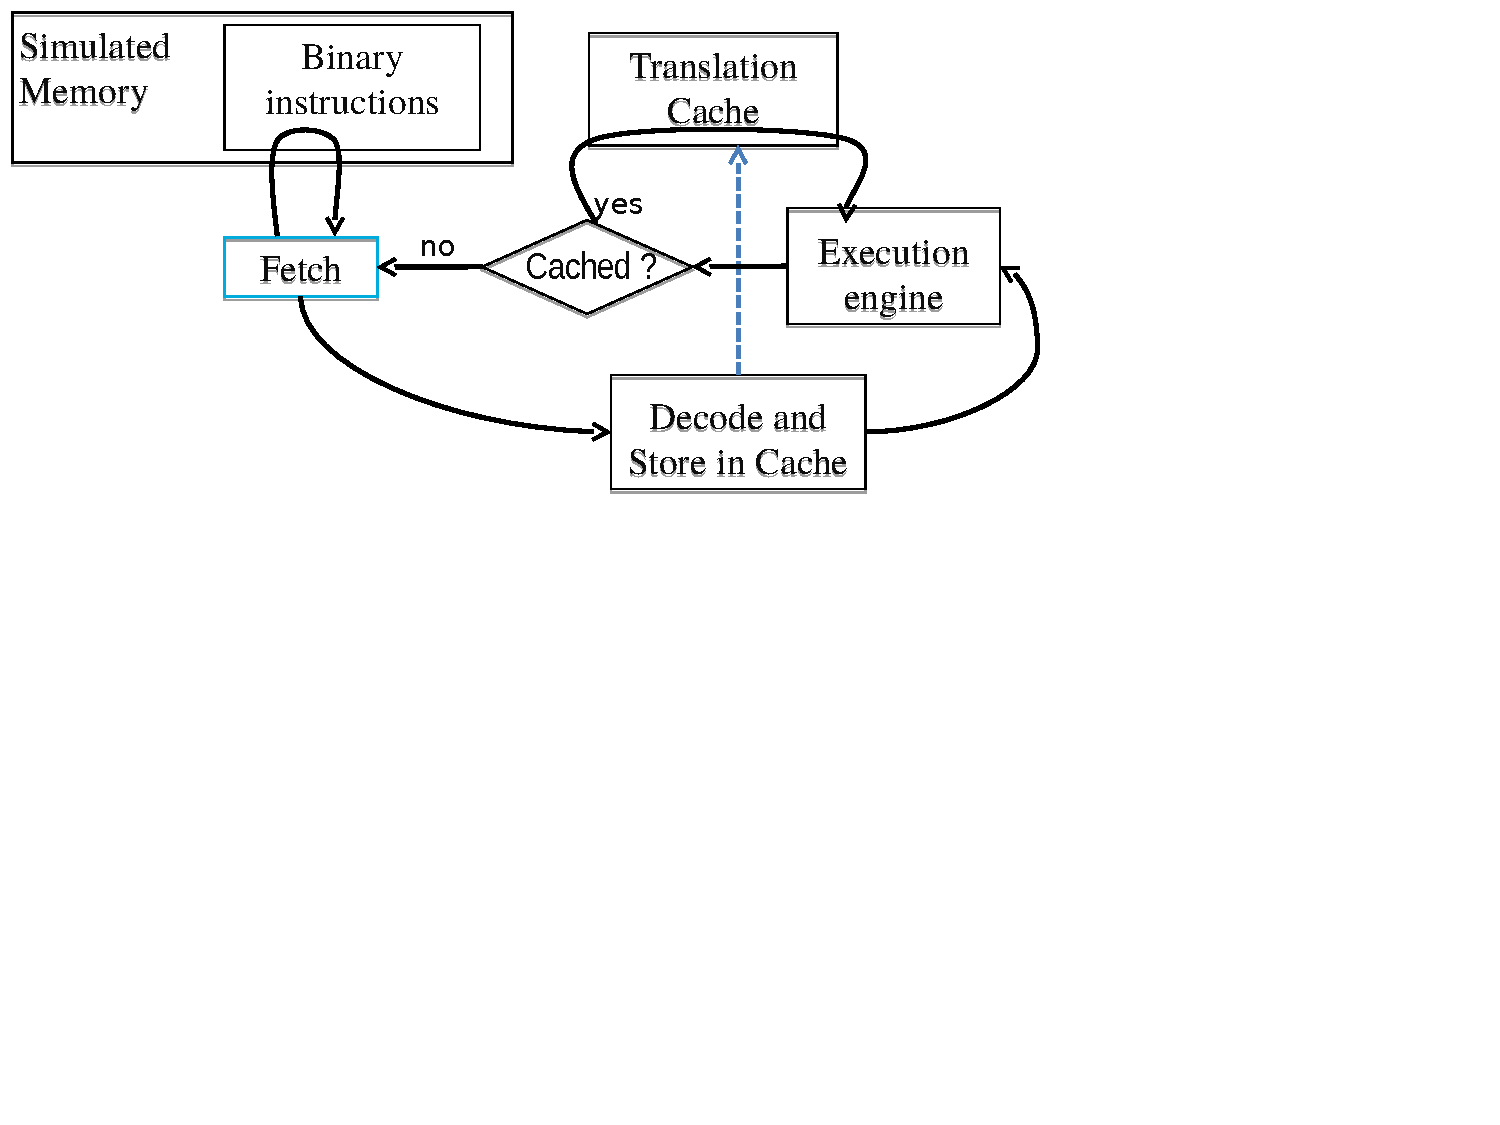
\includegraphics[scale=0.5, trim= 0mm 105mm 25mm 2mm, clip=true]
{fig/dyntrans.pdf}
  \caption{Dynamic Binary Translation}
  \label{fig:iss}
\end{figure}
With dynamic binary cached translation, illustrated in
Figure~\ref{fig:iss}, the target instructions are fetched from memory at
run-time but they are decoded only on the first execution and the
simulator translates these instructions into another representation,
which is stored into a cache. On further execution of the same
instructions, the translated cached version is used. If the code is
modified during run-time, the simulator invalidates the cached
representation.  Although dynamic translation introduces a compile
time phase as part of an overall simulation session, this translation
latency is amortized over time and it has been commonly used
\cite{shade-cmelik-keppel,embra-witchell-rosenblum,reshadi-mishra-dynamicISS,scott-kumar-retargetable,vala-duesterwald-dynamo}.

SimSoC belongs to the dynamic binary translation family of simulators.
In order to compare different techniques, and to provide different
levels of trade-offs of accuracy vs. speed, \simsoc implements four
modes of instruction simulation.  The first mode is interpretive
simulation.  This is the basis from which we can compare
performance. The second mode does dynamic binary translation using
{\em partial evaluation}, a compiling optimization technique, also
known as specialization~\cite{futamura}. Specialization can be
advantageously used in processor simulation, because data can often be
computed at instruction decoding time, and a specialized version of
the generic instruction can be used to execute it.  The simulation
code then uses fewer tests, fewer memory accesses and more immediate
instructions. This technique has been used to some extent in
\cite{naul-braun-jit-iccs} and usage of partial evaluation in \simsoc
is described in \cite{simsoc-csee2008} .

SimSoC dynamic translation uses an intermediate
representation that is partly dependent on the target architecture,
but does not involve the maintenance cost of a compiler.  A SimSoC ISS
includes pre-compiled code loaded at start-up time. The decoder
dynamically constructs an intermediate representation that maps the
binary instructions to this pre-compiled code. The decoding phase
mostly amounts to locating the appropriate code from the pre-compiled
library. In addition, the translator can construct the control flow
graph of the decoded software into linked basic blocks, and achieve
further optimization at block level.
\begin{figure}[h]
  \centering
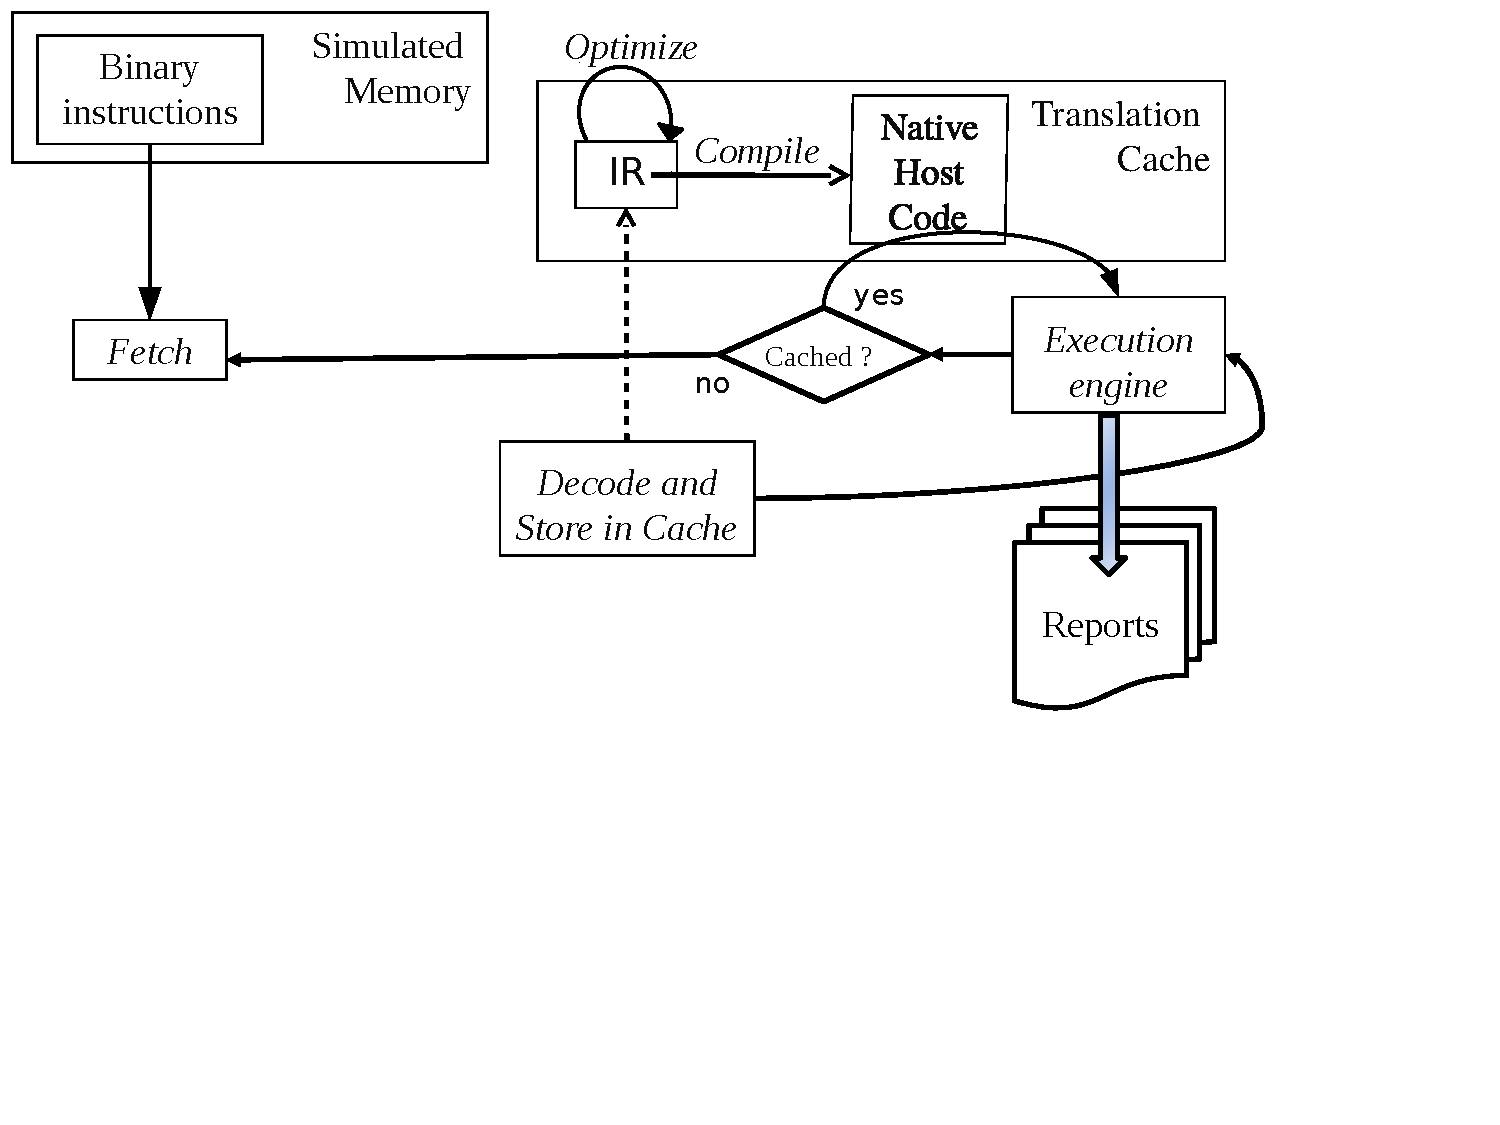
\includegraphics[scale=0.5, trim= 0mm 90mm 10mm 0mm, clip=true]
{fig/dyntrans-native.pdf}
  \caption{Dynamic Binary Translation}
  \label{fig:dyntrans-native}
\end{figure}

To increase simulation speed, yet another dynamic translation mode was
added later which uses the LLVM~\cite{llvm-2004} library to translate
on the fly target basic blocks into LLVM, yet again using a
pre-compiled library in LLVM bitcode.  Then one can use the existing
LLVM optimizer and Just-In-Time compiler to generate native code, as
shown in Figure~\ref{fig:dyntrans-native}.
The translation time from target code to LLVM, next from LLVM to
native, can become lengthy and ultimately defeat the speed-up in
execution time. Thus, the ISS actually mixes translation modes with a
method to evaluate and select only ``hot path'' code so that the LLVM
translation is not systematic, but only operates on such hot paths,
the remaining code being simulated with the standard translation. This
effectively provides overall faster simulation. We have also
experimented another mode with larger translation units, by
dynamically determining strongly coupled basic blocks in the control
flow graph. Finally, in order to benefit from multi-core simulation
hosts, a distributed dynamic translation mechanism has been
experimented.  In that configuration, the native code translation is
achieved by a separate dynamic translation server, that runs
concurrently with the ISS on other processors. This work has been
described in \cite{simsoc-llvm-2011} and \cite{amasbt-2012}.

\subsection{Performance Estimate}

SimSoC version released in open source is Loosely Timed. It advances
the clock using the quantum method. Each instruction is
assumed to execute in some time, which defaults to a constant
time. Each quantum of N instructions (a parameter) the clock is
advanced by the amount of execution time for that quantum. This method
makes it possible to run application software with timers and have
some idea of the software performance, but it cannot be used for worse
case analysis or fine grain performance estimates.

Recently, we have worked on a Approximately Timed version, with a
model of the instruction cache and the data cache and the pipe line,
for a sample of a Power architecture processor. These models are
abstract models, they do not mimic the architecture.  First the ISS
dynamic translator constructs the basic blocks. Next, for each basic
block an analysis is performed to compute its timing. Some of these
computations can be done statically only once, in particular the pipe
line stalls can be computed by a symbolic execution.  Also, it can be
determined at the entrance of a block whether the instruction cache
will miss or not, and only in that case compute the cache miss delay.
One still needs to execute the load store to check for cache miss, but
it is not necessary to physically cache the data. It is sufficient to
know which addresses are held in the cache. The computed information
can be stored as back annotation of the block for further usage.  This
work is described in \cite{witpress-2014} but is not yet part of the
open source code branch.


\subsection{Full System Simulators simulation}

\simsoc can fully simulate a hardware platform. In addition to the
ISS, it also includes implementation of several Memory Management
Units (MMU's). These MMU's are implemented as C++ subclass of a
generic abstract MMU defined in the infrastructure. The generic MMU
manages the TLB's and the details of the simulation of the target
memory using host memory. Particular implementations of MMU's have
been done for ARM, Power and MIPS chips. Similarly, a few interrupt
controllers have been implemented.

Since all of these simulation models are implemented as SystemC modules
using transaction modeling, one may elaborate complete platforms to
simulate a full system simulator running an operating system.  As a
proof of concept, we have developed several simulators to simulate
commercially available System-on-Chips. All of the SoC's we have
developed are running the Linux operating system, using the Linux
binary as is for the commercial chip. In order to boot Linux, it is
also possible to use a boot loader such as U-Boot.  The SoCs available
are:
\begin{itemize}
\item the SPEArPlus 600 circuit from ST Microelectronics.  This SoC
  contains among other components two ARM926 subsystems (dual core),
  together with various peripheral controllers.
\item the Texas Instrument AM1705 circuit. For this SoC, we have also
  developed an Ethernet controller model, and a bridge to real
  Internet so that we can test the simulated platform connected to
  real machines on the network, thanks to a bridge with the local
  Ethernet port.
\item the FreeScale 8641D dual core Power architecture chip.
\item We have under construction an example of the Power ez200 series,
for which we develop an Approximately Timed version.
\end{itemize}


%%%%%%%%%%%%%%%%%%%%%%%%%%%%%%%%%%%%%%%%%%%%%%%%%%%%%%%%%%%%%%%%%%%%%%%%%%%%%
\section{Certified Simulation}
\label{method}

A instruction set simulator is supposed to faithfully reproduce the
behavior of an instruction set architecture. But is this true ?
We have experimented a new approach to certify that a simulator
coded in C could be certified to be faithful to a processor model.
Our approach to obtain such a certified simulator is illustrated in
Figure~\ref{fig:diagram}. Considering the ARM architecture (Version
6), we need to have the following:
\begin{itemize}
\item a simulator of the ARM instruction set in C
  that we can obtain from the ARM Reference manual.
\item obtain formal operational semantics of that code. Given some
  source code in C, one can obtain through a certified compiler,
  namely \compcert C, the verified machine code, or alternatively the
  formal semantics of the compiled program constructed by \compcert.
\item prove, using a theorem prover, namely Coq, that the resulting
  ISS semantics indeed implement the ARM instruction set architecture,
  to verify that the semantics of the simulator accurately modifies
  the processor state at each step. For that, we need to prove that
  the results are compliant with a formal model of the ARM
  architecture.
\end{itemize}
\begin{figure}
\hfil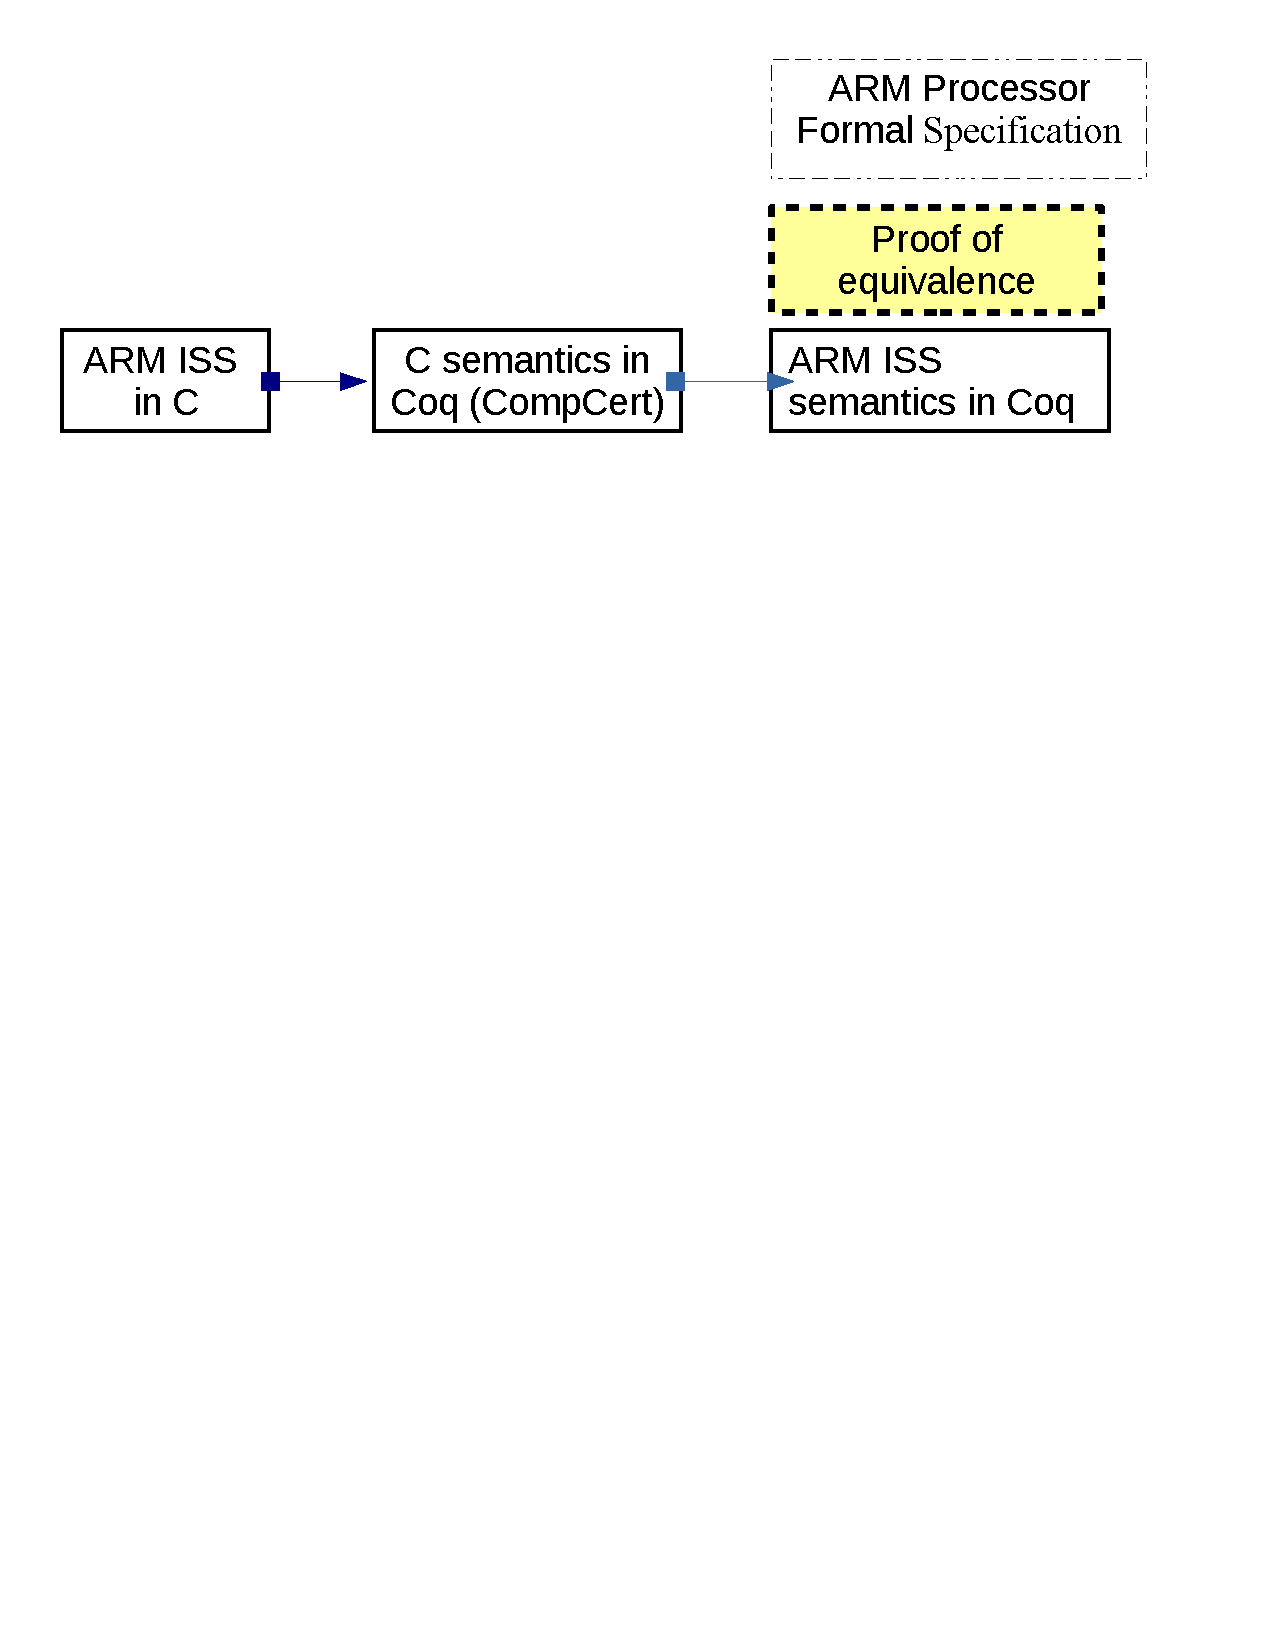
\includegraphics[scale=0.5, trim= 5mm 205mm 15mm 10mm, clip=true]
{fig/diagram.pdf}
\caption{Overall goal}
\label{fig:diagram}
\end{figure}
\subsection{Background}
\label{related}
Coq~\cite{coqart} is an interactive theorem prover. It allows the
expression of mathematical assertions and mechanically checks proofs
of these assertions.  Coq can also be presented as a dependently typed
$\lambda$-calculus or functional language.  For a detailed
presentation, the reader can consult~\cite{coqmanual}
or~\cite{coqart}. Coq is not an automated theorem prover: the logic
supported by Coq includes higher-order arithmetics, thus it is far too
rich to be decidable.  It is an interactive proof assistant that
requires human input to create appropriate auxiliary definitions,
choose the right inductive property and, more generally, to define the
architecture of the proof.  Automation is used for non-creative proof
steps and checking the correctness of the resulting formal proof.

\compcert is a formally verified compiler for the C programming
language provided by INRIA~\cite{ccc,Leroy-Compcert-CACM}.  Program
certification has to be based on a formal model of the program under
study.  Such a formal model is itself derived from a formal semantics
of the programming language. {\em Operational semantics} are used in
\compcert to define the execution of C programs.  The compiler is
specified, programmed, and proved in Coq. It has a complex translation
chain of multiple steps, from C source code into assembly code. It is
formally verified in the sense that the generated assembly code is
proved to behave exactly the same as the input program, according to a
formally defined operational semantics of the C language.  We
extensively use the C language formal operational semantics, from
which we get a formal model of the simulation program. We also use the
\compcert basic library, which defines formal data types for sequence
of bits, together with bit-wise operations and lemmas to describe their
properties.

There are 147 ARM instructions in the ARM V6 architecture.  For each
instruction, the manual provides its encoding table, its syntax, a
piece of pseudo-code explaining its own operation, its exceptions,
usage, and notes.  The simulator consists of two files extracted from
the manual: a \compcert C file to be linked with other components of
\simsoc (e.g memory access) and files representing each instruction in
\compcert C abstract syntax to be used for correctness proof.  There
is a standalone C function implementing each ARM instruction.  Each
function is composed of its return type, arguments variables, local
variables, and the function body. The body is a sequence of statements
including assignments and expressions, such as instruction \texttt{BL}
(\texttt{Branch and Link}): {\small
\begin{verbatim}
void B(struct SLv6_Processor *proc, const bool L,
       const SLv6_Condition cond, const uint32_t signed_immed_24){
 if (ConditionPassed(&proc->cpsr, cond)) {
   if (L == 1) set_reg(proc, 14, address_of_next_instruction(proc));
   set_pc_raw(proc, reg(proc,15)+(SignExtend_30(signed_immed_24)<<2));
}}
\end{verbatim}
}
\subsection{Approach}

In order to prove correctness, we need to have a formal model of the
ARM processor.  Ideally the formal specification of the ARM
architecture should be provided by the vendor. But it is not the case,
such a model is not available on their web site, hence we had
to build one. We chose to define a model of ARM architecture
in Coq, derived from the architecture reference manual
\cite{arm6refman}.
% As Coq models are executable,
%% No : Coq functional models are executable, but other models are not,
%% e.g., relational models as defined by an inductive relation
As our model is functional, it can be executed and tested
with real programs.

Starting from the C implementation of the ARM instruction set, we have
to prove that, given the initial state of the system, the execution of
an instruction as implemented by a C function results in the same
state as the formal specification. As each instruction is implemented
by a C function, we develop individual separate correctness
proofs.  The state of the ARM processor defined in the formal model is
called the \emph{abstract state}.  On the other hand, the same state
is represented by the data structures corresponding to C semantics
that we shall call the \emph{concrete state}.  In order to establish
correctness theorems we need to relate these two models.  Executing
the same instruction on the two sides produces a pair of new processor
states which should be related by the same correspondence. Informally,
executing the same instruction on a pair of equivalent states should
produce a new pair of equivalent states.
\begin{figure}
\hfil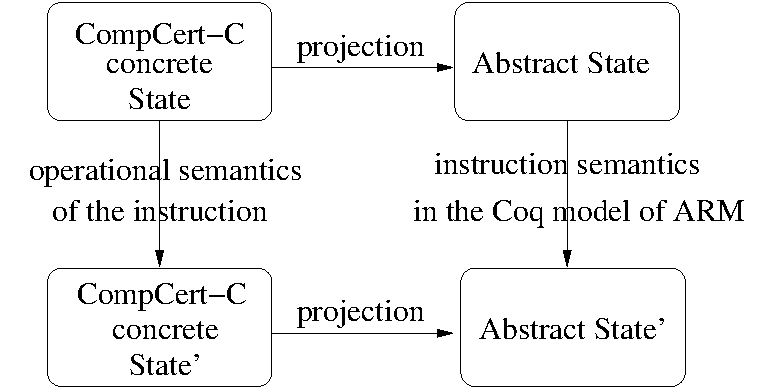
\includegraphics[width=.6\linewidth, trim= 2mm 0mm 2mm 0mm, clip=true]
{fig/theoremca.pdf}
\caption{Theorem statement for a given ARM instruction}
\label{fig:theoca}
\end{figure}
Our theorems are schematized by Figure~\ref{fig:theoca}. The complete
proofs are too lengthy for this workshop and have been given in
\cite{phd-xiaomu}.
%% JF : proections were better introduced below
% First we define suitable projections from the concrete state to the abstract state.
% as represented in Figure~\ref{fig:proj}.
To state the correctness theorem, we compare the \compcert C semantics
of a function corresponding to an ARM instruction with
the corresponding abstract definition.
%%
%% concrete side
%%
The processor states in the C implementation model are
complex, not only due to the inherent complexity of the C language
memory model, but also because of optimization and design decisions
targeting efficiency. For example, the C implementation uses embedded
\emph{struct}'s to express the ARM processor state.
According to the \compcert C semantics, the \emph{concrete state}
is represented based on a complex memory model with load and store functions
that are used for read/write operations over variables.
We also need to observe the modification of certain blocks of memory
corresponding to local variables.
%Re-using the \compcert C
%operational semantics, we are able to formally express the semantics
%of the C implementation of the ARM processor.
% \begin{figure}
% \hfil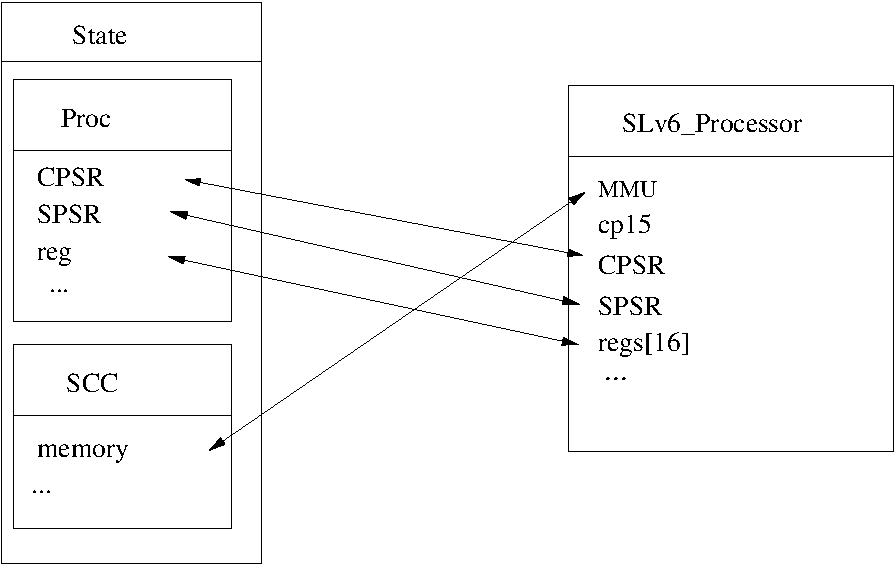
\includegraphics[width=.75\linewidth]{fig/proj.pdf}
% \caption{Projection}
% \label{fig:proj}
% \end{figure}
%%
%% abstract side
%%
%The proofs start from the abstract state described by the formal specification.
In the abstract Coq model, the processor state is kept as simple as possible.
%that can be directly used as the \emph{abstract state}.
%%
%% projection
%%
The main strategy is to define a projection which maps
the \emph{concrete state}
to the \emph{abstract state}.
%On both sides, the execution of an instruction is described
%by a state transition.
% In order to verify
% the projection of the pair of original states, we need to map the C
% memory state into a formal model.
%% JF: the next sentence is a "redite"
% On the concrete side, the state
% representations introduce a complex memory model, especially the
% memory representation of the processor state.
This projection uses elements from the local environment
as described by the \compcert C formalized memory model.
%% JF: old sentence
% Using the \compcert C formalized memory model, we have all
% elements ready to make the projection from the local environment to
% the abstract state to verify their equivalence.

Next, we need to consider the execution of the instruction.  The
semantics are defined as a relation between an initial expression and
an output expression after evaluation.  Then the body of the function
is executed.  On the abstract side, the new processor state is
obtained by running the formal model.  On the \compcert C side, the
execution is yielding a new memory state. We have to verify that the
projection from the concrete state does provide the same abstract
state.

Each proof is performed in a top-down manner. It follows the
definition of the instruction. %, analyzing the function step by step.
The function body is split into statements and then into expressions.
The ARM instruction execution is performed step by step.  When
evaluating an expression, we consider two kinds of information: (i)
how the memory state changes on \compcert C side; (ii) whether the
results on the abstract and the concrete model are related by the
projection.
%% JF: 2 next sentences peu informatives
% To this effect, we had to demonstrate a number of
% lemmas. With these lemmas, we can build the proof scripts for ARM
% instructions.
To discover the relation between memory states before and after
evaluating the C code, we have to {\em invert} the hypotheses of
operational semantics to follow the clue given by its definition, to
verify the hypotheses relating concrete memory states according to the
operational semantics. In order to reduce the proofs size and get
better maintainability, we studied a general solution to this problem,
and developed a new inversion tactics in Coq. With this new tactics,
the size of the proofs has become smaller and the proof scripts are
more manageable. The size vary with the instructions complexity from
170 lines for instruction LDRB (Load Register with Byte) to over 1200
for ADC (Add with Carry).  As a result, for each ARM instruction, we
can establish a theorem proving that the C code simulating an ARM
instruction is equivalent to the formal specification of the ARM
processor. All of these lemmas and theorems are verified by the Coq
theorem prover.  This work has been described in more detail in
\cite{monin:hal-00937168,rapido-2011}.

We acknowledge a weak point in our chain, due to the fact that the
hardware vendors do not provide formal semantics of their instruction
set. Because such formal models are unavailable, we had to define a
formal model of the ARM processor ourselves, which may be incorrect.
As Coq specifications are executable, we have been able to validate
our ARM formal model by checking that we obtain identical results with
real test programs, but this is not a formal proof... If the vendors
would make public formal specifications of their architectures, then
our tool chain could become fully verified.

\section{Conclusion}
\label{conclusion}

The SimSoC virtual prototyping software is a full system simulation
framework. Based on SystemC and TLM, it contains fast instruction set
simulators and a library of models for other hardware components such
as RS232 controller, or network controllers. Thanks to TLM interfaces,
these models can interact with other third party models to elaborate
complete simulation platforms that can run an operating system
starting from a bootloader.

We have added to SimSoc a proven generated simulator of the ARM
instruction set.  Given that we have a proof that the machine code
generated from C is correct, thanks to \compcert, and now a proof of
the ARM instruction set for these instructions, we have a proof that
the simulation of an algorithm on our simulator is conforming to the
algorithm for the target architecture.  With this technique, there is
no limit on the size of the C code that can be certified.  In fact, if
there existed a publicly available formal model of the ARM processor
approved by ARM Ltd company, our work, combined with \compcert C
compiler, could be construed to define a {\em certified execution of a
  C program}, that could be used for certification procedures.

\subsection{Acknowledgements}
This work has been partly funded by the international collaboration support
of France ANR and NSFC China in the SIVES project.

\bibliographystyle{splncs03}
\bibliography{references}

\end{document}
